\documentclass[twoside]{book}

% Packages required by doxygen
\usepackage{fixltx2e}
\usepackage{calc}
\usepackage{doxygen}
\usepackage[export]{adjustbox} % also loads graphicx
\usepackage{graphicx}
\usepackage[utf8]{inputenc}
\usepackage{makeidx}
\usepackage{multicol}
\usepackage{multirow}
\PassOptionsToPackage{warn}{textcomp}
\usepackage{textcomp}
\usepackage[nointegrals]{wasysym}
\usepackage[table]{xcolor}

% NLS support packages
\usepackage{polski}
\usepackage[T1]{fontenc}

% Font selection
\usepackage[T1]{fontenc}
\usepackage[scaled=.90]{helvet}
\usepackage{courier}
\usepackage{amssymb}
\usepackage{sectsty}
\renewcommand{\familydefault}{\sfdefault}
\allsectionsfont{%
  \fontseries{bc}\selectfont%
  \color{darkgray}%
}
\renewcommand{\DoxyLabelFont}{%
  \fontseries{bc}\selectfont%
  \color{darkgray}%
}
\newcommand{\+}{\discretionary{\mbox{\scriptsize$\hookleftarrow$}}{}{}}

% Page & text layout
\usepackage{geometry}
\geometry{%
  a4paper,%
  top=2.5cm,%
  bottom=2.5cm,%
  left=2.5cm,%
  right=2.5cm%
}
\tolerance=750
\hfuzz=15pt
\hbadness=750
\setlength{\emergencystretch}{15pt}
\setlength{\parindent}{0cm}
\setlength{\parskip}{0.2cm}
\makeatletter
\renewcommand{\paragraph}{%
  \@startsection{paragraph}{4}{0ex}{-1.0ex}{1.0ex}{%
    \normalfont\normalsize\bfseries\SS@parafont%
  }%
}
\renewcommand{\subparagraph}{%
  \@startsection{subparagraph}{5}{0ex}{-1.0ex}{1.0ex}{%
    \normalfont\normalsize\bfseries\SS@subparafont%
  }%
}
\makeatother

% Headers & footers
\usepackage{fancyhdr}
\pagestyle{fancyplain}
\fancyhead[LE]{\fancyplain{}{\bfseries\thepage}}
\fancyhead[CE]{\fancyplain{}{}}
\fancyhead[RE]{\fancyplain{}{\bfseries\leftmark}}
\fancyhead[LO]{\fancyplain{}{\bfseries\rightmark}}
\fancyhead[CO]{\fancyplain{}{}}
\fancyhead[RO]{\fancyplain{}{\bfseries\thepage}}
\fancyfoot[LE]{\fancyplain{}{}}
\fancyfoot[CE]{\fancyplain{}{}}
\fancyfoot[RE]{\fancyplain{}{\bfseries\scriptsize Wygenerowano Cz, 29 sty 2015 00\+:16\+:25 dla Biblioteka programem Doxygen }}
\fancyfoot[LO]{\fancyplain{}{\bfseries\scriptsize Wygenerowano Cz, 29 sty 2015 00\+:16\+:25 dla Biblioteka programem Doxygen }}
\fancyfoot[CO]{\fancyplain{}{}}
\fancyfoot[RO]{\fancyplain{}{}}
\renewcommand{\footrulewidth}{0.4pt}
\renewcommand{\chaptermark}[1]{%
  \markboth{#1}{}%
}
\renewcommand{\sectionmark}[1]{%
  \markright{\thesection\ #1}%
}

% Indices & bibliography
\usepackage{natbib}
\usepackage[titles]{tocloft}
\setcounter{tocdepth}{3}
\setcounter{secnumdepth}{5}
\makeindex

% Hyperlinks (required, but should be loaded last)
\usepackage{ifpdf}
\ifpdf
  \usepackage[pdftex,pagebackref=true]{hyperref}
\else
  \usepackage[ps2pdf,pagebackref=true]{hyperref}
\fi
\hypersetup{%
  colorlinks=true,%
  linkcolor=blue,%
  citecolor=blue,%
  unicode%
}

% Custom commands
\newcommand{\clearemptydoublepage}{%
  \newpage{\pagestyle{empty}\cleardoublepage}%
}


%===== C O N T E N T S =====

\begin{document}

% Titlepage & ToC
\hypersetup{pageanchor=false,
             bookmarks=true,
             bookmarksnumbered=true,
             pdfencoding=unicode
            }
\pagenumbering{roman}
\begin{titlepage}
\vspace*{7cm}
\begin{center}%
{\Large Biblioteka \\[1ex]\large 1.\+0 }\\
\vspace*{1cm}
{\large Wygenerowano przez Doxygen 1.8.9.1}\\
\vspace*{0.5cm}
{\small Cz, 29 sty 2015 00:16:25}\\
\end{center}
\end{titlepage}
\clearemptydoublepage
\tableofcontents
\clearemptydoublepage
\pagenumbering{arabic}
\hypersetup{pageanchor=true}

%--- Begin generated contents ---
\chapter{Indeks hierarchiczny}
\section{Hierarchia klas}
Ta lista dziedziczenia posortowana jest z grubsza, choć nie całkowicie, alfabetycznie\+:\begin{DoxyCompactList}
\item \contentsline{section}{biblioteka.\+Biblioteka}{\pageref{classbiblioteka_1_1_biblioteka}}{}
\item \contentsline{section}{model.\+Czytelnik}{\pageref{classmodel_1_1_czytelnik}}{}
\item \contentsline{section}{Jdbc\+Test}{\pageref{class_jdbc_test}}{}
\item J\+Frame\begin{DoxyCompactList}
\item \contentsline{section}{biblioteka.\+Main\+Panel}{\pageref{classbiblioteka_1_1_main_panel}}{}
\end{DoxyCompactList}
\item \contentsline{section}{model.\+Ksiazka}{\pageref{classmodel_1_1_ksiazka}}{}
\item \contentsline{section}{model.\+Wypozyczenie}{\pageref{classmodel_1_1_wypozyczenie}}{}
\end{DoxyCompactList}

\chapter{Indeks klas}
\section{Lista klas}
Tutaj znajdują się klasy, struktury, unie i interfejsy wraz z ich krótkimi opisami\+:\begin{DoxyCompactList}
\item\contentsline{section}{\hyperlink{classbiblioteka_1_1_biblioteka}{biblioteka.\+Biblioteka} }{\pageref{classbiblioteka_1_1_biblioteka}}{}
\item\contentsline{section}{\hyperlink{classmodel_1_1_czytelnik}{model.\+Czytelnik} }{\pageref{classmodel_1_1_czytelnik}}{}
\item\contentsline{section}{\hyperlink{class_jdbc_test}{Jdbc\+Test} }{\pageref{class_jdbc_test}}{}
\item\contentsline{section}{\hyperlink{classmodel_1_1_ksiazka}{model.\+Ksiazka} }{\pageref{classmodel_1_1_ksiazka}}{}
\item\contentsline{section}{\hyperlink{classbiblioteka_1_1_main_panel}{biblioteka.\+Main\+Panel} }{\pageref{classbiblioteka_1_1_main_panel}}{}
\item\contentsline{section}{\hyperlink{classmodel_1_1_wypozyczenie}{model.\+Wypozyczenie} }{\pageref{classmodel_1_1_wypozyczenie}}{}
\end{DoxyCompactList}

\chapter{Dokumentacja klas}
\hypertarget{classbiblioteka_1_1_biblioteka}{}\section{Dokumentacja klasy biblioteka.\+Biblioteka}
\label{classbiblioteka_1_1_biblioteka}\index{biblioteka.\+Biblioteka@{biblioteka.\+Biblioteka}}
\subsection*{Metody publiczne}
\begin{DoxyCompactItemize}
\item 
\hypertarget{classbiblioteka_1_1_biblioteka_aec6840e69d3f1fb90bc10923a54ea05d}{}boolean {\bfseries create\+Tables} ()\label{classbiblioteka_1_1_biblioteka_aec6840e69d3f1fb90bc10923a54ea05d}

\item 
\hypertarget{classbiblioteka_1_1_biblioteka_a543eca0bfd67c61dc67ab8c00a55d615}{}boolean {\bfseries insert\+Czytelnik} (String imie, String nazwisko, String pesel)\label{classbiblioteka_1_1_biblioteka_a543eca0bfd67c61dc67ab8c00a55d615}

\item 
\hypertarget{classbiblioteka_1_1_biblioteka_aa11038d7dc6b4c3c105f8fd522012e98}{}boolean {\bfseries insert\+Ksiazka} (String tytul, String autor)\label{classbiblioteka_1_1_biblioteka_aa11038d7dc6b4c3c105f8fd522012e98}

\item 
\hypertarget{classbiblioteka_1_1_biblioteka_a7d441e9629d5df4fead45666bd608596}{}boolean {\bfseries insert\+Wypozycz} (int id\+Czytelnik, int id\+Ksiazka)\label{classbiblioteka_1_1_biblioteka_a7d441e9629d5df4fead45666bd608596}

\item 
\hypertarget{classbiblioteka_1_1_biblioteka_ae3008a6f5ec7c42cb9ce051c70b882c5}{}boolean {\bfseries delete\+Wypozycz} (int id\+Czytelnik, int id\+Ksiazka)\label{classbiblioteka_1_1_biblioteka_ae3008a6f5ec7c42cb9ce051c70b882c5}

\item 
\hypertarget{classbiblioteka_1_1_biblioteka_ad6ac7eb8ee418e42d6932af5726e8e45}{}List$<$ \hyperlink{classmodel_1_1_czytelnik}{Czytelnik} $>$ {\bfseries select\+Czytelnicy} ()\label{classbiblioteka_1_1_biblioteka_ad6ac7eb8ee418e42d6932af5726e8e45}

\item 
\hypertarget{classbiblioteka_1_1_biblioteka_a59e88d76a498f36be2c0e7611cc1d598}{}List$<$ \hyperlink{classmodel_1_1_ksiazka}{Ksiazka} $>$ {\bfseries select\+Ksiazki} ()\label{classbiblioteka_1_1_biblioteka_a59e88d76a498f36be2c0e7611cc1d598}

\item 
\hypertarget{classbiblioteka_1_1_biblioteka_a95c5a33e87a81142b908fc14cf2a97df}{}List$<$ \hyperlink{classmodel_1_1_wypozyczenie}{Wypozyczenie} $>$ {\bfseries select\+Rezerwacja} ()\label{classbiblioteka_1_1_biblioteka_a95c5a33e87a81142b908fc14cf2a97df}

\item 
\hypertarget{classbiblioteka_1_1_biblioteka_a576871df6ce74a8ab03d612d503fc1dc}{}void {\bfseries close\+Connection} ()\label{classbiblioteka_1_1_biblioteka_a576871df6ce74a8ab03d612d503fc1dc}

\end{DoxyCompactItemize}
\subsection*{Statyczne atrybuty publiczne}
\begin{DoxyCompactItemize}
\item 
\hypertarget{classbiblioteka_1_1_biblioteka_ae76ee0ce4adb34be329935dbdab51983}{}static final String {\bfseries D\+R\+I\+V\+E\+R} = \char`\"{}org.\+sqlite.\+J\+D\+B\+C\char`\"{}\label{classbiblioteka_1_1_biblioteka_ae76ee0ce4adb34be329935dbdab51983}

\item 
\hypertarget{classbiblioteka_1_1_biblioteka_a1dd6b10f95302c5cd0148aaee71bfb8d}{}static final String {\bfseries D\+B\+\_\+\+U\+R\+L} = \char`\"{}jdbc\+:sqlite\+:biblioteka.\+db\char`\"{}\label{classbiblioteka_1_1_biblioteka_a1dd6b10f95302c5cd0148aaee71bfb8d}

\end{DoxyCompactItemize}


Dokumentacja dla tej klasy została wygenerowana z pliku\+:\begin{DoxyCompactItemize}
\item 
C\+:/\+Users/\+Mateusz/\+Desktop/\+S\+T\+U\+D\+I\+A/\+Projekt-\/\+Inzynieria-\/\+Oprogramowania/\+J\+D\+B\+C\+Project v2/src/biblioteka/Biblioteka.\+java\end{DoxyCompactItemize}

\hypertarget{classmodel_1_1_czytelnik}{}\section{Dokumentacja klasy model.\+Czytelnik}
\label{classmodel_1_1_czytelnik}\index{model.\+Czytelnik@{model.\+Czytelnik}}
\subsection*{Metody publiczne}
\begin{DoxyCompactItemize}
\item 
\hypertarget{classmodel_1_1_czytelnik_a350c5cbcc8ed36a73b64ae53d9bed261}{}int {\bfseries get\+Id} ()\label{classmodel_1_1_czytelnik_a350c5cbcc8ed36a73b64ae53d9bed261}

\item 
\hypertarget{classmodel_1_1_czytelnik_abb528a96cc894cbc16184453b3687200}{}void {\bfseries set\+Id} (int id)\label{classmodel_1_1_czytelnik_abb528a96cc894cbc16184453b3687200}

\item 
\hypertarget{classmodel_1_1_czytelnik_a0901e0710b3eac9be263fe0b9fc4ee28}{}String {\bfseries get\+Imie} ()\label{classmodel_1_1_czytelnik_a0901e0710b3eac9be263fe0b9fc4ee28}

\item 
\hypertarget{classmodel_1_1_czytelnik_aaf30f5f126f186d3505b1ff4e722c586}{}void {\bfseries set\+Imie} (String imie)\label{classmodel_1_1_czytelnik_aaf30f5f126f186d3505b1ff4e722c586}

\item 
\hypertarget{classmodel_1_1_czytelnik_a47ef0cd71c0e198b89b1bb2b4ceff75e}{}String {\bfseries get\+Nazwisko} ()\label{classmodel_1_1_czytelnik_a47ef0cd71c0e198b89b1bb2b4ceff75e}

\item 
\hypertarget{classmodel_1_1_czytelnik_ab14283d96648d14ea23db6be3be56540}{}void {\bfseries set\+Nazwisko} (String nazwisko)\label{classmodel_1_1_czytelnik_ab14283d96648d14ea23db6be3be56540}

\item 
\hypertarget{classmodel_1_1_czytelnik_a9a682c40c4310a06b532357a979a9c41}{}String {\bfseries get\+Pesel} ()\label{classmodel_1_1_czytelnik_a9a682c40c4310a06b532357a979a9c41}

\item 
\hypertarget{classmodel_1_1_czytelnik_a545b138589f94038b09dce5e55b2b78b}{}void {\bfseries set\+Pesel} (String pesel)\label{classmodel_1_1_czytelnik_a545b138589f94038b09dce5e55b2b78b}

\item 
\hypertarget{classmodel_1_1_czytelnik_a46e86f825bde67387bf61b10893db16d}{}{\bfseries Czytelnik} (int id, String imie, String nazwisko, String pesel)\label{classmodel_1_1_czytelnik_a46e86f825bde67387bf61b10893db16d}

\item 
\hypertarget{classmodel_1_1_czytelnik_afdcdd5b3496717892836107722b287b2}{}String {\bfseries to\+String} ()\label{classmodel_1_1_czytelnik_afdcdd5b3496717892836107722b287b2}

\end{DoxyCompactItemize}


Dokumentacja dla tej klasy została wygenerowana z pliku\+:\begin{DoxyCompactItemize}
\item 
C\+:/\+Users/\+Mateusz/\+Desktop/\+S\+T\+U\+D\+I\+A/\+Projekt-\/\+Inzynieria-\/\+Oprogramowania/\+J\+D\+B\+C\+Project v2/src/model/Czytelnik.\+java\end{DoxyCompactItemize}

\hypertarget{class_jdbc_test}{}\section{Dokumentacja klasy Jdbc\+Test}
\label{class_jdbc_test}\index{Jdbc\+Test@{Jdbc\+Test}}
\subsection*{Statyczne metody publiczne}
\begin{DoxyCompactItemize}
\item 
\hypertarget{class_jdbc_test_a87e08226bd87e253e364287100408f80}{}static void {\bfseries main} (String\mbox{[}$\,$\mbox{]} args)\label{class_jdbc_test_a87e08226bd87e253e364287100408f80}

\end{DoxyCompactItemize}


Dokumentacja dla tej klasy została wygenerowana z pliku\+:\begin{DoxyCompactItemize}
\item 
C\+:/\+Users/\+Mateusz/\+Desktop/\+S\+T\+U\+D\+I\+A/\+Projekt-\/\+Inzynieria-\/\+Oprogramowania/\+J\+D\+B\+C\+Project v2/src/Jdbc\+Test.\+java\end{DoxyCompactItemize}

\hypertarget{classmodel_1_1_ksiazka}{}\section{Dokumentacja klasy model.\+Ksiazka}
\label{classmodel_1_1_ksiazka}\index{model.\+Ksiazka@{model.\+Ksiazka}}
\subsection*{Metody publiczne}
\begin{DoxyCompactItemize}
\item 
\hypertarget{classmodel_1_1_ksiazka_a7457258b6900580a2782d4a1f961d585}{}int {\bfseries get\+Id} ()\label{classmodel_1_1_ksiazka_a7457258b6900580a2782d4a1f961d585}

\item 
\hypertarget{classmodel_1_1_ksiazka_a299b97510c645087185b6f9a1ee63ff6}{}void {\bfseries set\+Id} (int id)\label{classmodel_1_1_ksiazka_a299b97510c645087185b6f9a1ee63ff6}

\item 
\hypertarget{classmodel_1_1_ksiazka_ab0eaf84ec1b2d7da641b5f8cc6379fa2}{}String {\bfseries get\+Tytul} ()\label{classmodel_1_1_ksiazka_ab0eaf84ec1b2d7da641b5f8cc6379fa2}

\item 
\hypertarget{classmodel_1_1_ksiazka_a143d2f509f17dfce2b52860ee703eb06}{}void {\bfseries set\+Tytul} (String tytul)\label{classmodel_1_1_ksiazka_a143d2f509f17dfce2b52860ee703eb06}

\item 
\hypertarget{classmodel_1_1_ksiazka_ae513998c41e1e3e0987c6305c660e1d3}{}String {\bfseries get\+Autor} ()\label{classmodel_1_1_ksiazka_ae513998c41e1e3e0987c6305c660e1d3}

\item 
\hypertarget{classmodel_1_1_ksiazka_ad31e02240487cea80ad86a1f8cf30f9c}{}void {\bfseries set\+Autor} (String autor)\label{classmodel_1_1_ksiazka_ad31e02240487cea80ad86a1f8cf30f9c}

\item 
\hypertarget{classmodel_1_1_ksiazka_af3da0dea16a09266879ed6884ec71b3f}{}{\bfseries Ksiazka} (int id, String tytul, String autor)\label{classmodel_1_1_ksiazka_af3da0dea16a09266879ed6884ec71b3f}

\item 
\hypertarget{classmodel_1_1_ksiazka_aaca5aa304ed7ffd753d2eda6ecfb12b4}{}String {\bfseries to\+String} ()\label{classmodel_1_1_ksiazka_aaca5aa304ed7ffd753d2eda6ecfb12b4}

\end{DoxyCompactItemize}


Dokumentacja dla tej klasy została wygenerowana z pliku\+:\begin{DoxyCompactItemize}
\item 
C\+:/\+Users/\+Mateusz/\+Desktop/\+S\+T\+U\+D\+I\+A/\+Projekt-\/\+Inzynieria-\/\+Oprogramowania/\+J\+D\+B\+C\+Project v2/src/model/Ksiazka.\+java\end{DoxyCompactItemize}

\hypertarget{classbiblioteka_1_1_main_panel}{}\section{Dokumentacja klasy biblioteka.\+Main\+Panel}
\label{classbiblioteka_1_1_main_panel}\index{biblioteka.\+Main\+Panel@{biblioteka.\+Main\+Panel}}
Diagram dziedziczenia dla biblioteka.\+Main\+Panel\begin{figure}[H]
\begin{center}
\leavevmode
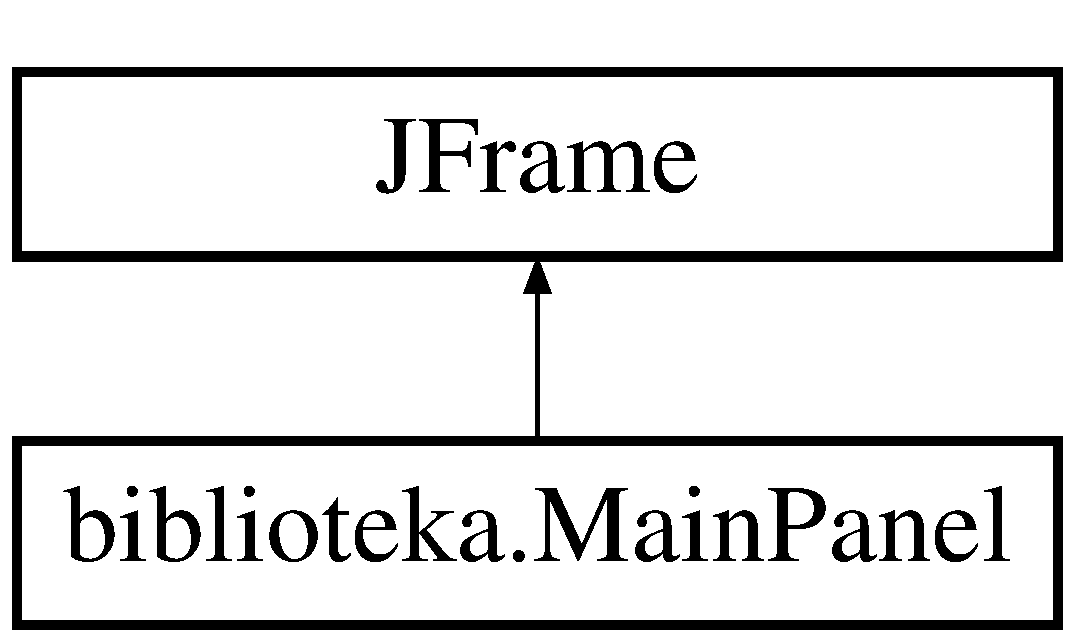
\includegraphics[height=2.000000cm]{classbiblioteka_1_1_main_panel}
\end{center}
\end{figure}
\subsection*{Metody publiczne}
\begin{DoxyCompactItemize}
\item 
\hypertarget{classbiblioteka_1_1_main_panel_a44f32e074f14c0fff8a5400db110ba33}{}void {\bfseries add\+Dodaj\+Ksiazke\+Listener} (Action\+Listener listener)\label{classbiblioteka_1_1_main_panel_a44f32e074f14c0fff8a5400db110ba33}

\item 
\hypertarget{classbiblioteka_1_1_main_panel_a74f4bacecbde8fcf47b9d4a80aa268e2}{}void {\bfseries add\+Dodaj\+Czytelnika\+Listener} (Action\+Listener listener)\label{classbiblioteka_1_1_main_panel_a74f4bacecbde8fcf47b9d4a80aa268e2}

\item 
\hypertarget{classbiblioteka_1_1_main_panel_a0fd3cae160a97892c23c0acbfaf33e07}{}void {\bfseries show\+Base\+Listener} (Action\+Listener listener)\label{classbiblioteka_1_1_main_panel_a0fd3cae160a97892c23c0acbfaf33e07}

\item 
\hypertarget{classbiblioteka_1_1_main_panel_a22918328747985b73c275f7989b8d0dd}{}void {\bfseries rezerwacja\+Listener} (Action\+Listener listener)\label{classbiblioteka_1_1_main_panel_a22918328747985b73c275f7989b8d0dd}

\item 
\hypertarget{classbiblioteka_1_1_main_panel_a0a1019eab5d8867eca875d8a45b4f150}{}void {\bfseries usun\+Rezerwacje\+Listener} (Action\+Listener listener)\label{classbiblioteka_1_1_main_panel_a0a1019eab5d8867eca875d8a45b4f150}

\item 
\hypertarget{classbiblioteka_1_1_main_panel_aa63ec952c009506c84c237a99eb685b2}{}String {\bfseries get\+Tytul\+Ksiazki} ()\label{classbiblioteka_1_1_main_panel_aa63ec952c009506c84c237a99eb685b2}

\item 
\hypertarget{classbiblioteka_1_1_main_panel_a427ee72cd6fa7c5f52c955f8a7fae151}{}String {\bfseries get\+Autor\+Ksiazki} ()\label{classbiblioteka_1_1_main_panel_a427ee72cd6fa7c5f52c955f8a7fae151}

\item 
\hypertarget{classbiblioteka_1_1_main_panel_a5e9c92d9da979560029f94cc140ab358}{}String {\bfseries get\+Imie\+Czytelnika} ()\label{classbiblioteka_1_1_main_panel_a5e9c92d9da979560029f94cc140ab358}

\item 
\hypertarget{classbiblioteka_1_1_main_panel_a6b72aa36a3f2a239aada12e18cc7e4e6}{}String {\bfseries get\+Nazwisko\+Czytelnika} ()\label{classbiblioteka_1_1_main_panel_a6b72aa36a3f2a239aada12e18cc7e4e6}

\item 
\hypertarget{classbiblioteka_1_1_main_panel_a7926942fab384f46a47715541c7453a0}{}String {\bfseries get\+Pesel\+Czytelnika} ()\label{classbiblioteka_1_1_main_panel_a7926942fab384f46a47715541c7453a0}

\item 
\hypertarget{classbiblioteka_1_1_main_panel_abb6488bbff6634725243a49b7c84565f}{}String {\bfseries get\+Id\+Czytelnika} ()\label{classbiblioteka_1_1_main_panel_abb6488bbff6634725243a49b7c84565f}

\item 
\hypertarget{classbiblioteka_1_1_main_panel_a820b99c1e7198374658ba0ddc4258468}{}String {\bfseries get\+Id\+Ksiazki} ()\label{classbiblioteka_1_1_main_panel_a820b99c1e7198374658ba0ddc4258468}

\item 
\hypertarget{classbiblioteka_1_1_main_panel_a2c89b9c82d26e77706285cc40e6eb738}{}String {\bfseries get\+Id\+Czytelnika\+Do\+Usuniecia} ()\label{classbiblioteka_1_1_main_panel_a2c89b9c82d26e77706285cc40e6eb738}

\item 
\hypertarget{classbiblioteka_1_1_main_panel_a3fca1630118b1147c6fbeecabfbf8be3}{}String {\bfseries get\+Id\+Ksiazki\+Do\+Usuniecia} ()\label{classbiblioteka_1_1_main_panel_a3fca1630118b1147c6fbeecabfbf8be3}

\end{DoxyCompactItemize}
\subsection*{Metody chronione}
\begin{DoxyCompactItemize}
\item 
\hypertarget{classbiblioteka_1_1_main_panel_a9890e804a7aa7696432964d188e28bb5}{}void {\bfseries init\+Ksiazka\+Text\+Box} ()\label{classbiblioteka_1_1_main_panel_a9890e804a7aa7696432964d188e28bb5}

\item 
\hypertarget{classbiblioteka_1_1_main_panel_ab68776d6f01edc5eb496b92da19a50c1}{}void {\bfseries init\+Button} (String nazwa)\label{classbiblioteka_1_1_main_panel_ab68776d6f01edc5eb496b92da19a50c1}

\item 
\hypertarget{classbiblioteka_1_1_main_panel_a2c7a3da68e5a1071c46f60788afc50eb}{}void {\bfseries init\+Location} ()\label{classbiblioteka_1_1_main_panel_a2c7a3da68e5a1071c46f60788afc50eb}

\end{DoxyCompactItemize}
\subsection*{Statyczne atrybuty chronione}
\begin{DoxyCompactItemize}
\item 
\hypertarget{classbiblioteka_1_1_main_panel_ad35e2ebd0df24b1e86d863bdc73facdd}{}static int {\bfseries D\+E\+F\+A\+U\+L\+T\+\_\+\+W\+I\+D\+T\+H} = 400\label{classbiblioteka_1_1_main_panel_ad35e2ebd0df24b1e86d863bdc73facdd}

\item 
\hypertarget{classbiblioteka_1_1_main_panel_a9c4ce53d69777e541fc122459d61bf77}{}static int {\bfseries D\+E\+F\+A\+U\+L\+T\+\_\+\+H\+E\+I\+G\+H\+T} = 700\label{classbiblioteka_1_1_main_panel_a9c4ce53d69777e541fc122459d61bf77}

\end{DoxyCompactItemize}


Dokumentacja dla tej klasy została wygenerowana z pliku\+:\begin{DoxyCompactItemize}
\item 
C\+:/\+Users/\+Mateusz/\+Desktop/\+S\+T\+U\+D\+I\+A/\+Projekt-\/\+Inzynieria-\/\+Oprogramowania/\+J\+D\+B\+C\+Project v2/src/biblioteka/Main\+Panel.\+java\end{DoxyCompactItemize}

\hypertarget{classmodel_1_1_wypozyczenie}{}\section{Dokumentacja klasy model.\+Wypozyczenie}
\label{classmodel_1_1_wypozyczenie}\index{model.\+Wypozyczenie@{model.\+Wypozyczenie}}
\subsection*{Metody publiczne}
\begin{DoxyCompactItemize}
\item 
\hypertarget{classmodel_1_1_wypozyczenie_a39c3dd6fffd0a74d906129f854285395}{}int {\bfseries get\+Id\+Ksiazka} ()\label{classmodel_1_1_wypozyczenie_a39c3dd6fffd0a74d906129f854285395}

\item 
\hypertarget{classmodel_1_1_wypozyczenie_a9f4e45419040b7d3e76c9d912bafd318}{}void {\bfseries set\+Id\+Ksiazka} (int id\+Ksiazka)\label{classmodel_1_1_wypozyczenie_a9f4e45419040b7d3e76c9d912bafd318}

\item 
\hypertarget{classmodel_1_1_wypozyczenie_af979983b3d4687f8f2b90b153019233d}{}int {\bfseries get\+Id\+Czytelnik} ()\label{classmodel_1_1_wypozyczenie_af979983b3d4687f8f2b90b153019233d}

\item 
\hypertarget{classmodel_1_1_wypozyczenie_ae2d2d4b72c182a3d858a623d759e61bf}{}void {\bfseries set\+Id\+Czytelnik} (int id\+Czytelnik)\label{classmodel_1_1_wypozyczenie_ae2d2d4b72c182a3d858a623d759e61bf}

\item 
\hypertarget{classmodel_1_1_wypozyczenie_ad480eeab4a795e8892a877c7bbf5818f}{}{\bfseries Wypozyczenie} (int id\+Ksiazka, int id\+Czytelnik)\label{classmodel_1_1_wypozyczenie_ad480eeab4a795e8892a877c7bbf5818f}

\item 
\hypertarget{classmodel_1_1_wypozyczenie_a9e6df55be2c1d8e7dc49f0614cd0da56}{}{\bfseries Wypozyczenie} (int id, int id\+Ksiazka, int id\+Czytelnik)\label{classmodel_1_1_wypozyczenie_a9e6df55be2c1d8e7dc49f0614cd0da56}

\item 
\hypertarget{classmodel_1_1_wypozyczenie_ad0656f62fb92711844e3e6113df91473}{}String {\bfseries to\+String} ()\label{classmodel_1_1_wypozyczenie_ad0656f62fb92711844e3e6113df91473}

\end{DoxyCompactItemize}


Dokumentacja dla tej klasy została wygenerowana z pliku\+:\begin{DoxyCompactItemize}
\item 
C\+:/\+Users/\+Mateusz/\+Desktop/\+S\+T\+U\+D\+I\+A/\+Projekt-\/\+Inzynieria-\/\+Oprogramowania/\+J\+D\+B\+C\+Project v2/src/model/Wypozyczenie.\+java\end{DoxyCompactItemize}

%--- End generated contents ---

% Index
\backmatter
\newpage
\phantomsection
\clearemptydoublepage
\addcontentsline{toc}{chapter}{Indeks}
\printindex

\end{document}
